\documentclass[12pt,a4paper]{article}
\usepackage[left=2.5cm,right=2cm,top=2cm,bottom=2cm]{geometry}
\usepackage{tabularx}
\usepackage{setspace}
\usepackage{graphicx}
\usepackage{array}
\usepackage{fancyhdr}
\usepackage{times}


\pagestyle{fancy}
\renewcommand{\headrulewidth}{0pt}
\fancyhf{}
\rfoot{\thepage}

\setlength{\parindent}{0pt}
\renewcommand{\arraystretch}{1.25}

\begin{document}

\begin{center}
{\Large \textbf{RIWAYAT HIDUP}}
\end{center}

\vspace{0.5cm}

%==============================%
% BIODATA DIRI
%==============================%
\textbf{BIODATA DIRI}
\vspace{0.2cm}
\hrule
\vspace{0.5cm}

\noindent
\begin{minipage}{0.70\textwidth}
\begin{tabularx}{\textwidth}{p{3.8cm} l X}
Binusian ID         & : & 2502121162 \\
Nama                & : & Frans Sebastian \\
Tempat/Tanggal Lahir & : & Wonogiri / 25 April 2003 \\
Jenis Kelamin       & : & Laki-laki \\
Email               & : & frans.sebastian@binus.ac.id
 \\
\end{tabularx}
\end{minipage}
\hfill
\begin{minipage}{0.28\textwidth}
\begin{center}
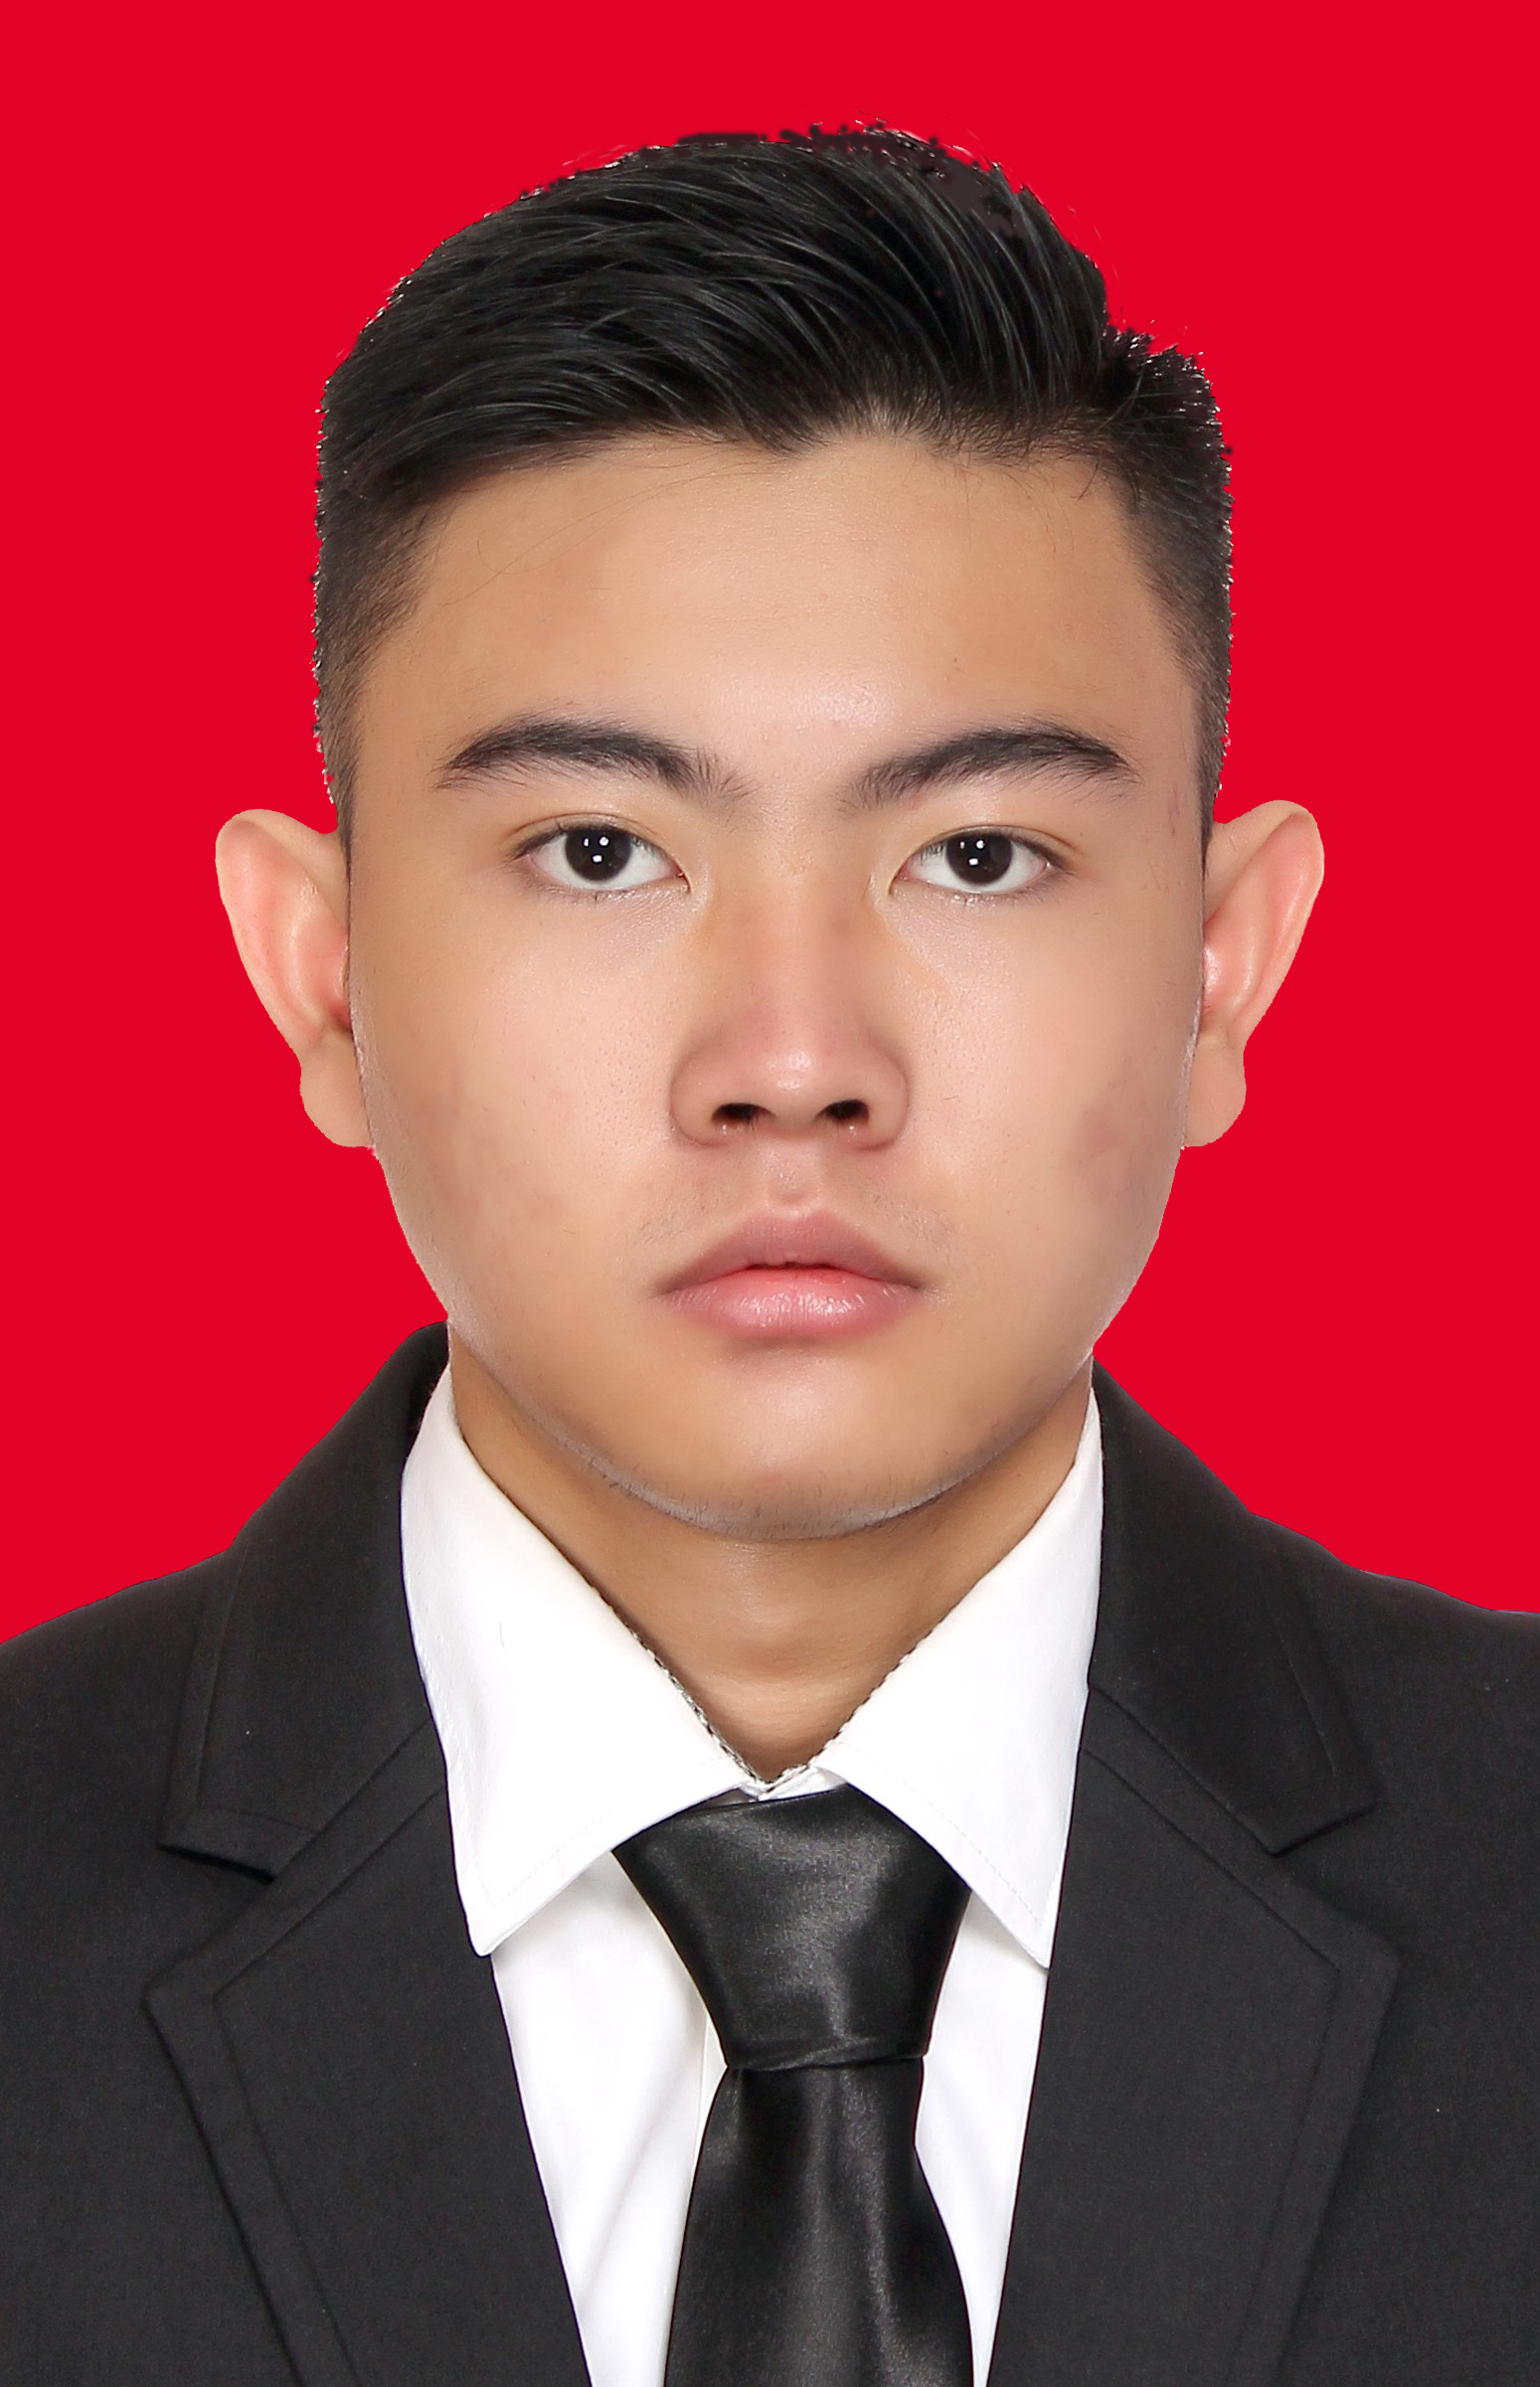
\includegraphics[width=3cm]{Graduation Photo.jpg}
\end{center}
\end{minipage}

%---- Alamat dan data lanjutan tanpa foto mengganggu ----%
\vspace{0.4cm}

\begin{tabularx}{\textwidth}{p{3.8cm} l X}
Alamat              & : &
\textbf{Domisili:} Jl. Aries Utama No.50, RT.3/RW.3, Meruya Utara, Kec. Kembangan, Kota Jakarta Barat, Daerah Khusus Ibukota Jakarta 11620 \\
& &
\textbf{Permanen:} RT 003 / RW 003, Dusun Sawahan, Desa Ploso, Kecamatan Purwantoro, Kabupaten Wonogiri, Jawa Tengah, 57695 \\
No. HP              & : & 085217095294 \\
Kewarganegaraan     & : & Indonesia \\
Status Perkawinan   & : & Belum Kawin \\
Agama               & : & Katholik \\
\end{tabularx}

\vspace{0.8cm}
%==============================%
% RIWAYAT PENDIDIKAN
%==============================%
\textbf{RIWAYAT PENDIDIKAN}
\vspace{0.2cm}
\hrule
\vspace{0.5cm}

\textbf{Pendidikan Saat Ini}
\begin{tabbing}
\hspace{4cm} \= \hspace{10cm} \kill
Pendidikan Saat Ini \> : Strata 1 \\
Nama Sekolah \> : Universitas Bina Nusantara \\
Jurusan \> : S1 Teknik Informatika \\
Periode \> : 2022 - sekarang \\
GPA (sementara) \> : 3.87 / 4 \\
\end{tabbing}

\vspace{0.3cm}

\textbf{Pendidikan Terakhir}
\begin{tabbing}
\hspace{4cm} \= \hspace{10cm} \kill
Pendidikan Terakhir \> : SMA \\
Nama Sekolah \> : SMA Kristen Filadelfia Sadaniang  \\
Jurusan \> : IPA \\
Periode \> : 2018 - 2021 \\
\end{tabbing}


%==============================%
% PENGALAMAN ORGANISASI
%==============================%
% \vspace{0.5cm}
% \textbf{PENGALAMAN ORGANISASI}
% \vspace{0.2cm}
% \hrule
% \vspace{0.4cm}

% \textbf{Himpunan Mahasiswa Mekatronika Otomasi (HIMAMO) / 2016–2019} \\
% Anggota Bidang Kaderisasi (2017–2019) \\
% Periode keanggotaan: 2016–2019

% \vspace{0.3cm}

% \textbf{Unit Kegiatan Mahasiswa Seni Budaya Minangkabau (UKM-SBM) / 2016–2019} \\
% Anggota Seni Randai (2016–2018) \\
% Ketua UKM–SBM (2018–2019) \\
% Periode keanggotaan: 2016–2019

%==============================%
% SERTIFIKASI PERSONAL
%==============================%
\vspace{0.5cm}
\textbf{SERTIFIKASI PERSONAL}
\vspace{0.2cm}
\hrule
\vspace{0.4cm}

\textbf{Machine Learning A-Z Hands-On Python And R In Data Science} / \textit{Udemy} \\
\textit{Online Course} dengan total durasi 44.5 jam, diselesaikan pada 29 Januaryi 2022.

\vspace{2cm}

%==============================%
% PENGALAMAN KERJA
%==============================%
\vspace{0.5cm}
\textbf{PENGALAMAN KERJA}
\vspace{0.2cm}
\hrule
\vspace{0.4cm}

\textbf{Kredivo Group -- PT Finaccel Teknologi Indonesia} \\
\textit{Machine Learning Engineer} \\
Agustus 2024 - Sekarang \\
Bertanggung jawab membuat program machine learning dan \textit{system design} untuk credit \textit{risk approval}, serta memastikan semua model berjalan dengan baik.
\vspace{0.3cm}

\textbf{Gradana Indonesia -- PT Gradana Teknoruci Indonesia} \\
\textit{Senior Software Engineer} \\
Juli 2023 - Agustus 2024 \\
Bertanggung jawab membuat program software web dan \textit{system design} untuk credit \textit{risk approval}, login, transaksi dan integrasi vendor serta memastikan semua web berjalan dengan baik.
\vspace{0.3cm}

\textbf{(Silvertech Asia | Brandztory)-- PT Primatek Infokom Jaya} \\
\textit{Software Engineer} \\
Januari 2022 - April 2022 \\
Bertanggung jawab membuat program software web, mobile dan server untuk login, transaksi dan integrasi vendor serta memastikan semua web berjalan dengan baik.
\vspace{0.3cm}

\textbf{Egafood Indonesia -- PT Egafood Multi Cipta} \\
\textit{Full-stack Developer} \\
October 2021 - Januari 2022 \\
Bertanggung jawab membuat program software web profil perusahaan serta memastikan web berjalan dengan baik.
\vspace{0.3cm}

% %==============================%
% % PENGHARGAAN
% %==============================%
% \vspace{0.5cm}
% \textbf{PENGHARGAAN DAN PRESTASI}
% \vspace{0.2cm}
% \hrule
% \vspace{0.4cm}

% \textbf{Prestasi Akademik – Universitas Bina Nusantara (BINUS) @Bekasi} \\
% Meraih Indeks Prestasi Kumulatif (IPK) Tertinggi di Program Studi Ilmu Komputer untuk periode 2221 (Diterbitkan pada Mei 2023).



\end{document}